\documentclass[15pt]{ctexart}
\usepackage{xeCJK}
	\setCJKmainfont{SimSun}         % 缺省中文字体为宋体
	\setmainfont{Times New Roman}   % 缺省英文字体 Times New Roman
\usepackage{geometry}
	\geometry{bottom=3.5cm}
\usepackage{float}
\usepackage{listings}
\usepackage{graphicx}
\usepackage{appendix}	
\usepackage[colorlinks]{hyperref}
\usepackage{amsmath}
\usepackage{indentfirst}
\usepackage{enumerate}
\usepackage{fancyhdr}
\usepackage{textcomp}
\usepackage{appendix} 
\usepackage{multirow}
\usepackage{geometry}
\geometry{verbose,letterpaper}
\usepackage{media9}
\pagestyle{fancy}
\lhead{虚拟路由}
\rhead{\thepage}
\cfoot{}
\lstset{frameshape={RYRYNYYYY}{yny}{yny}{RYRYNYYYY}, backgroundcolor=\color[RGB]{245,245,244}}

\begin{document}
\begin{titlepage}
    \centering
    
\includegraphics[scale=0.9]{imgs/SYSULogo.png}\par\vspace{1cm}
    \vspace{1cm}
    {\scshape\huge 虚拟路由 \\ 项目报告 \\ \centering \scshape \Huge 模拟网络层路由 \par}
    \vspace{1.5cm}
    {\Large\bfseries \flushleft 学院:数据科学与计算机学院 \\ 专业:计算机科学与技术 \\ 年级:2016级 \\组长(学号):王锡淮(16337236)\\组员(学号):杨陈泽(16337271)\\
    组员(学号):肖遥(16337258)\par}
    % \vspace{2cm}

% Bottom of the page
    % {\large \today\par}
\end{titlepage}
\tableofcontents
\newpage
\section{项目介绍} % (fold)
\label{sec:项目介绍}
	模拟网络层路由项目包含三个部分:
	\begin{enumerate}
		\item 基本RIP协议
		\item 基本OSPF协议
		\item 基本中心化路由协议实现
	\end{enumerate}
	\par 在其中的每一个部分中,都实现了基本的路由功能以及对于基本算法缺点和不足的改进,比如,在基本RIP协议中,使用split-horizon、poison-inverse,holddown方法和triggered update方法缓解了无穷计数问题;在基本OSPF协议中,实现了多条等费用路径的路由选择,并且解决了路由循环问题和改善了路由震荡问题;在中心化路由协议中使用Twisted异步编程框架以减轻服务器进程的资源消耗;等等。项目中3个部分使用的都是UDP协议以传输路由信息,使用UDP也节约了网络资源。
	\par 项目主页见\url{https://github.com/Leo-xh/Virtual-Routing}。
% section 项目介绍 (end)
\section{基本RIP协议} % (fold)
\label{sec:rip}
	\subsection{协议概述} % (fold)
	\label{sub:协议概述}
		本项目中实现的RIP协议采用了RIPv1和RIPv2的协议规定的一部分,是一个基于DV算法的网络层路由协议。其主要算法是Bellman-Ford算法,路由费用以路由跳数作为度量,运行该协议的每个路由器能够计算出到其余路由器的下一跳路由以及路由费用。定义了请求报文和响应报文两种报文格式。为了尽可能避免环路和无穷计数问题,使用的机制包括毒性逆转(split-horizon with poison inverse)、延时刷新(flush timer)、触发更新(triggered update)、抑制更新(holddown)。在协议的扩展中,实现了该协议下适用的traceRoute功能。
	% subsection 协议概述 (end)
	\subsection{算法} % (fold)
	\label{sub:算法}
		\subsubsection{距离矢量表更新}
		\label{ssub:距离矢量表更新}
		距离矢量表计算主要基于Bellman-Ford算法。在基本的DV算法中,路由器每次收到邻居发来的距离矢量时,会使用Bellman-Ford的更新公式更新自己的距离矢量表:$$ dist_{self}(dest) = \min_{neighbour}\{dist_{neighbour}(dest) + metric(self,neighbour)\} $$ 为此,路由器需要在维护自己距离矢量表的同时,保存邻居发来的距离矢量表。
		\par 在RIP协议中,路由器只需保存和维护自己的距离矢量表。在收到邻居发来的距离矢量时,会将其与自己当前的距离矢量表进行比较,而不是用所有邻居的距离矢量表重新计算和比较。具体而言,RIP协议使用的更新公式为(假设收到邻居$nb$的距离矢量):$$ dist_{self}(dest) = \begin{cases} \min( dist_{self}(dest), dist_{nb}(dest) + metric(self,nb) ) & , nextHop_{self}(dest) \neq nb \\ dist_{nb}(dest) + metric(self,nb) & , nextHop_{self}(dest) = nb \end{cases}$$ 采用这种更新方式避免了路由器存储邻居距离矢量表的开销,也减少了更新所需的计算量。不足之处在于最短路径费用增加时,不能马上从其余路径中找到更优的并将其替代,需要等待其他邻居发送距离矢量。(事实上,为了避免环路和无穷计数问题,原最短路径费用增加后从其余路径中找替代的更新方式是不被允许的。)
		\subsubsection{环路与无限计数避免机制}
		\label{ssub:环路与无限计数避免机制}
		在本项目的实现中,为了尽可能避免环路与无限计数问题,使用了以下4种机制:
		\begin{itemize}
			\item 毒性逆转:一个路由器向邻居发的距离矢量中,下一跳为该邻居的项费用改为无穷(16)。
			\item 延迟刷新:一个路由器在与一个邻居失去连接(链路中断)后,不立即将其从距离矢量表中清除,而是延迟一段时间。在这段时间里,链路中断的信息能够告知其他路由。
			\item 触发更新:一个路由器在距离矢量表更新后,将更新的项立即向所有邻居发送。特别地,当一条链路断开后,触发更新会沿着包含这一链路的所有最短路径传播,从而使这些路径被毒化(即在路由器的转发表中费用为无穷)。
			\item 抑制更新:一个路由器在其一条最短路径被毒化后的一段时间内,忽略收到的一切声称能到达该路径目的地的距离矢量。这是为了避免在网络不稳定时使用邻居过时的路由信息进行更新。
		\end{itemize}
	% subsection 算法 (end)
	\subsection{协议特性} % (fold)
	\label{sub:协议特性}
	\subsubsection{协议流程} % (fold)
		\label{ssub:协议流程}
		本项目中实现的RIP协议主要包含的流程如下:
		\begin{itemize}
			\item 路由器在进入区域时,向所有邻居发送request报文,邻居则返回一个response报文,里面含有邻居的距离矢量表。
			\item 该路由器会定时地向所有的邻居发送response报文,即自己的距离矢量表。
			\item 收到一个response报文意味着要维持该邻居的状态;而如果在一段时间内没有收到某个邻居路由器的response报文,则认为与该路由器的链路中断。
			\item 当收到其它邻居路由器的距离矢量表时,根据该信息更新自己的距离矢量表;当自己的距离矢量更新时,向所有邻居发送自己新的距离矢量表(只发送更新的部分)。
		\end{itemize}
		% subsubsection 协议流程 (end)
	% subsection 协议特性 (end)
	\subsection{报文格式} % (fold)
	\label{sub:报文格式}
	本实验中使用的普通报文普通数据报文、request报文、response报文、TraceRoute报文、Echo报文如下:
	\par 普通报文:
	\begin{table}[H]
		\centering
		\begin{tabular}{|c|}
			\hline
			Command \\
			\hline
			source address \\
			\hline
			destination address \\
			\hline
			payload \\
			\hline
		\end{tabular}		
	\end{table}
	request报文:
	\begin{table}[H]
		\centering
		\begin{tabular}{|c|}
			\hline
			Command \; \vline \; Version \; \vline \; Routing domain \; \\
			\hline
			Source address \\
			\hline
			Address family \; \vline \; Route tag \; \\
			\hline
			address \\
			\hline
			Next hop \\
			\hline
			metric \\
			\hline
		\end{tabular}
	\end{table}
	Response报文:
	\begin{table}[H]
		\centering
		\begin{tabular}{|c|}
			\hline
			Command \; \vline \; Version \; \vline \; Routing domain \; \\
			\hline
			Source address \\
			\hline
			Address family \; \vline \; Route tag \; \\
			\hline
			address \\
			\hline
			Next hop \\
			\hline
			metric \\
			\hline
			repeat of last 17 bytes \\
			\hline
			$\cdots$ \\
			\hline 
		\end{tabular}	
	\end{table}
	TraceRoute报文:
	\begin{table}[H]
	\centering
		\begin{tabular}{|c|}
			\hline
			Command \\
			\hline
			source address \\
			\hline
			destination address \\
			\hline
			count \\
			\hline
		\end{tabular}		
	\end{table}	
	Echo 报文:
	\begin{table}[H]
	\centering
		\begin{tabular}{|c|}
			\hline
			Command \\
			\hline
			source address \\
			\hline
			destination address \\
			\hline
			local address \\
			\hline
		\end{tabular}		
	\end{table}
	报文项解释:
	\begin{enumerate}
		\item Command(1 Byte):指明这条报文的类型。
		\begin{enumerate}[]
			\item 0:普通报文。
			\item 1:请求报文。
			\item 2:响应(包含路由表)报文。
			\item 3:TraceRoute报文。
			\item 4:Echo报文。
		\end{enumerate}
		\item Version(1 Byte):RIP协议的版本。
		\item Routing domain(2 Bytes):指明这是RIP中的哪一步。
		\item Source address(6 Bytes):指明发送方的源地址和监听端口。
		\item Address family(2 Bytes):使用什么作为地址,使用IP该项为2。
		\item Route tag(2 Bytes):本项目中不用。
		\item address(6 Bytes):ip和端口号。
		\item Next hop(6 Bytes):下一跳路由的ip和端口。
		\item metric(1 Byte):代价度量(跳数)。
		\item Local address(6 Bytes):指明Echo报文发送者的源地址和监听端口。
		\item Count(1 Byte):路由跳数。
	\end{enumerate}
	% subsection 报文格式 (end)
	\subsection{协议扩展} % (fold)
	\label{sub:协议扩展}
		\begin{enumerate}
			\item 网络环路\\
				路由器可能收到自己发送的路由信息,因此造成网络环路。\\
				为了避免该情况,采用了:毒性逆转、抑制更新和触发更新等机制。
			\item 无穷计数\\
				·采用延迟刷新,在检测到一个邻居可能失效时不立即将其从数据库中删除,等待一个间隔后再删除,目的是通告其它邻居该失效邻居不可达。
			\item TraceRoute\\
				·基于RIP路由16跳不可达这一机理,向目的地发跳数为1-16共16个报文,当一个路由器收到该报文,则提取其中的跳数,并将它减一。\\
				·当跳数为0时,向报文的源地址返回一个Echo报文;否则将跳数打包进原报文中,继续向目的地转发。\\
				·源地址路由器收集所有返回的Echo报文,如果5s内收到目的地址返回的Echo报文,则输出该路径;否则认为该目的地址不可达。
		\end{enumerate}
	% subsection 协议扩展 (end)
	\subsection{协议实现} % (fold)
	\label{sub:协议实现}
		本RIP协议基本由Python实现,主要利用的是socket库进行套接字编程并采用的是UDP协议、struct库进行数据的打包和解包、threading库管理线程和定时器。
		\par 实现方法实现了一个RIP协议类,处理内部流程和为外部调用留出了收发数据、查询路由路径等接口。
	% subsection 协议实现 (end)
	\subsection{结果} % (fold)
	\label{sub:结果}
		测试所用的拓扑图以及路由结果如下图\ref{fig:ripTest1}和\ref{fig:ripTest2}所示。
		\begin{figure}[H]
			\centering
			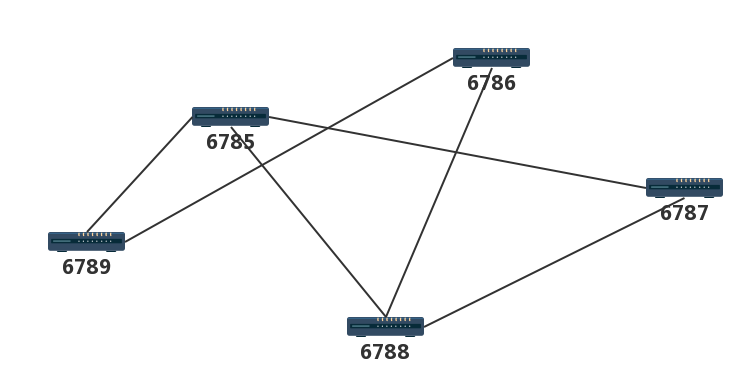
\includegraphics[scale=0.4]{imgs/topo1/tpop1.png}
			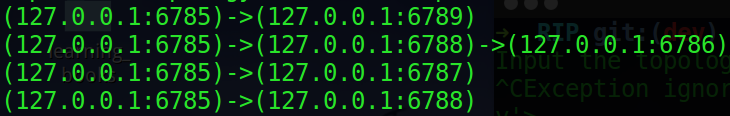
\includegraphics[scale=0.5]{imgs/ripTest1.PNG}
			\caption{RIP测试样例一}
			\label{fig:ripTest1}
		\end{figure}
		\begin{figure}[H]
			\centering
			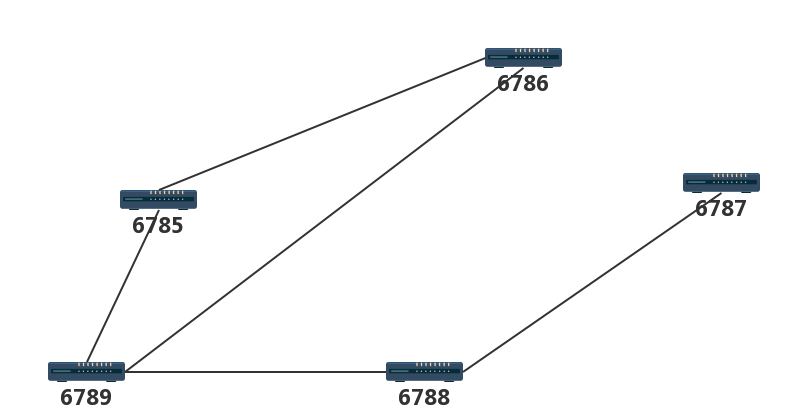
\includegraphics[scale=0.4]{imgs/topo1/topo2.png}
			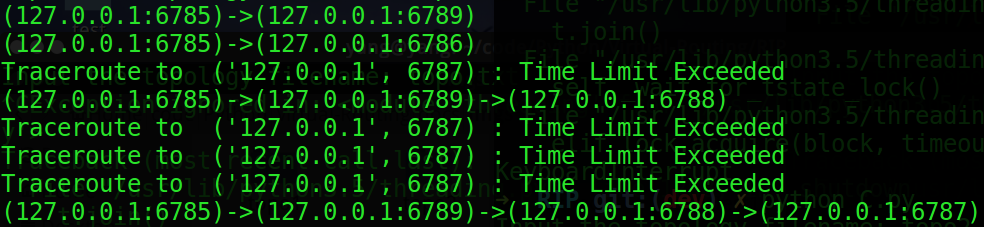
\includegraphics[scale=0.4]{imgs/ripTest2.PNG}
			\caption{RIP测试样例二}
			\label{fig:ripTest2}
		\end{figure}
		成功找出了其中的跳数最小的路径。
	% subsection 结果 (end)
	\subsection{总结} % (fold)
	\label{sub:总结}
		\begin{enumerate}
			\item 原生的DV算法会因为RIP收敛速度缓慢,而产生路由环路的问题,而我们的RIP协议中采用了多种机制来解决了这种问题。
			\item 原生的DV算法需要保存邻居的路由表,而采用RIP协议的更新公式,避免了路由器存储邻居路由表的开销,而且减少了路由器更新时的计算量。
		\end{enumerate}
	
	% subsection 总结 (end)


% section rip (end)
\section{基本OSPF协议} % (fold)
\label{sec:ospf}
	\subsection{协议概述} % (fold)
	\label{sub:协议概述}
		本项目中实现的OSPF协议是一个基于链路状态的路由协议,运行该协议的每个路由器能够根据收到的所有链路信息计算出一个最短路径树,构造对应的转发表。其链路的权重的赋值取决于带宽,算法使用的是Dijkstra算法和RPF广播算法,定义了Hello和LS(link-state)两种报文格式。实现了多条等费用路径的路由选择,并且解决了路由循环问题和改善了路由震荡问题。在协议的扩展中,实现了该协议下适用的traceRoute功能。
	% subsection 协议概述 (end)
	\subsection{算法} % (fold)
	\label{sub:算法}
		\subsubsection{路由计算算法} % (fold)
		\label{ssub:路由计算算法}
			在原生LS算法中,一个路由器的路由计算的方法是:以自身为起点,执行Dijkstra算法以得到一棵最短路径树,然后根据最短路径树得到转发表。采用这种方法,计算出的到每个目的地的最短路径是唯一的。
			\par 为了实现多条等费用最短路径选择,本项目采用以下算法过程:
			\begin{itemize}
				\item 对于路由器的每个邻居$nb$,以$nb$为起点执行Dijkstra算法,得到$nb$到其他路由器的最短路径距离$dist_{nb}$。
				\item 使用Bellman-Ford更新公式,计算自身到其他路由器的距离:$$dist_{self}(dest) = \min_{nb}\{dist_{nb}(dest) + metric(self,nb)\} $$
				\item 对于每一个目的地$dest$,依次判断每个邻居是否能作为下一跳(即该邻居是否在一条最短路径上)。判断一个邻居$nb$能作为下一跳的依据是:$nb$能到达$dest$并且满足公式$$dist_{self}(dest) = dist_{nb}(dest) + metric(self,nb)$$将符合条件的邻居加入转发表中去往$dest$的下一跳列表。
			\end{itemize}		
		% subsubsection 路由计算算法 (end)
		\subsubsection{广播算法} % (fold)
		\label{ssub:广播算法}
			使用了RPF(Reverse Path First)算法,收到一个广播数据包的路由器会向来路以外的路由器转发该广播数据包当且仅当来路位于广播源和当前路有器的任一条最短路径上。
		% subsubsection 广播算法 (end)
	% subsection 算法 (end)
	\subsection{协议特性} % (fold)
	\label{sub:协议特性}
		\subsubsection{协议流程} % (fold)
		\label{ssub:协议流程}
		本项目中实现的OSPF协议主要包含的流程如下:
		\begin{enumerate}
			\item 路由器在进入区域时,向所有邻居发送hello报文(该报文用于向邻居声明自己的存在),再向该区域内的路由器广播自己的链路信息。
			\item 该路由器会定时地发送hello报文和广播链路信息。
			\item 收到一个hello报文意味着要维持该邻居的状态;而如果在一段时间内没有收到某个邻居路由器的hello报文,则认为该路由器故障或离开该区域。
			\item 当自身的链路信息发生改变时,广播链路信息;当收到其它路由器的链路信息时,根据该信息更新自己的关于该区域的链路信息数据库。
		\end{enumerate}		
		% subsubsection 协议流程 (end)
	% subsection 协议特性 (end)
	\subsection{报文格式} % (fold)
	\label{sub:报文格式}
		该协议中包含的Hello报文、LS报文、traceRoute报文、Echo报文、普通数据报文格式如下:
		\par Hello 报文。
	\begin{table}[H]
	\centering
		\begin{tabular}{|c|}
			\hline
			Command \\
			\hline
			Source address \\
			\hline
			Metric \\
			\hline
		\end{tabular}		
	\end{table}

	LSU报文(广播报文)。
	\begin{table}[H]
	\centering
	\begin{tabular}{|c|}
		\hline                 
		Command                \\
		\hline                 
		Source address         \\
		\hline                 
		Transmit address       \\
		\hline                 
		Destination address    \\
		\hline                 
		Metric                 \\
		\hline                 
		Repeat of last 8 bytes \\
		\hline                 
		$\cdots$               \\
		\hline                 
	\end{tabular}		
\end{table}

TraceRoute报文
\begin{table}[H]
	\centering
	\begin{tabular}{|c|}
		\hline              
		Command             \\
		\hline              
		source address      \\
		\hline              
		destination address \\
		\hline              
		count               \\
		\hline              
	\end{tabular}		
\end{table}	

Echo 报文
\begin{table}[H]
	\centering
	\begin{tabular}{|c|}
		\hline              
		Command             \\
		\hline              
		source address      \\
		\hline              
		destination address \\
		\hline              
		local address       \\
		\hline              
	\end{tabular}		
\end{table}
普通报文的格式与在RIP中的格式相同。
报文项解释:
\begin{enumerate}[(1)]
	\item Command(1 Byte):指明这条报文的类型。
	      \begin{enumerate}[]
	      	\item 0: 普通报文
	      	\item 1: hello
	      	\item 2: LSU(Link State Update)
	      	\item 3: traceRoute
	      	\item 4: Echo
	      \end{enumerate}
	\item Source address(6 Bytes):指明发送方的源地址和监听端口。
	\item Destination address(6 Bytes):指明目的地的源地址和监听端口。
	\item Transmit address(6 Bytes):指明广播中转发者的源地址和监听端口。
	\item Local address(6 Bytes):指明Echo报文发送者的源地址和监听端口。
	\item Metric(2 Bytes):代价度量。
	\item Count(1 Bytes):路由跳数。
	\end{enumerate}
	
	% subsection 报文格式 (end)
	\subsection{协议扩展} % (fold)
	\label{sub:协议扩展}
		\begin{enumerate}
<<<<<<< HEAD
			\item 路由循环\\
				如果所有的节点都不在完全相同的地图上工作,则可以形成路由环路。 在这种情况下,最简单的形式是两个相邻节点都认为另一个节点是到达给定目的地的最佳路径。 任何到达任一节点的目的地的数据包将在两者之间循环。 涉及两个以上节点的路由环路也是可能的。
				\par 这是因为每个节点计算其最短路径树及其路由表而不与任何其他节点进行交互。 如果两个节点以不同的链路状态图启动,则可能会出现创建路由循环的情况。
				\par OSPF是一个无路由自环的协议,因为上述路由环路会在各个路由器重新通告并计算路径时消失。但是仍可以进一步优化。
				\par 本项目中的解决方法是路由器记录目前到达前10个的数据包的md5码,如果一个新到的数据包的md5码重复,则将其丢弃。选择10个而不是更多是因为数据包可能重传。
			\item 路由震荡\\
				为了避免路由震荡,设置路由器广播其链路信息的时间随机化。
			\item TraceRoute\\
				·由于OSPF没有跳数这一说法,向目的地发跳数为1-32共32个报文,当一个路由器收到该报文,则提取其中的跳数,并将它减一。\\
				·如果跳数为0,则向报文的源地址返回一个Echo报文;如果跳数>0且报文的目的地址不等于当前路由的地址,将跳数打包进原报文中,
				继续向目的地转发;否则,判定为多余的traceRoute报文,将之舍弃。\\
				·源地址路由器收集所有返回的Echo报文,如果5s内收到目的地址返回的Echo报文,则输出该路径;否则认为该目的地址不可达。
		\end{enumerate}
=======
			\item 路由循环
			\item 路由震荡
				\begin{itemize}
					\item 为了避免路由震荡,设置路由器广播其链路信息的时间随机化。
				\end{itemize}
			\item TraceRoute
				\begin{itemize}
					\item 由于OSPF没有跳数这一说法,向目的地发跳数为1-32共32个报文,当一个路由器收到该报文,则提取其中的跳数,并将它减一。\\
					\item 如果跳数为0,则向报文的源地址返回一个Echo报文;如果跳数>0且报文的目的地址不等于当前路由的地址,将跳数打包进原报文中,
					继续向目的地转发;否则,判定为多余的traceRoute报文,将之舍弃。\\
					\item 源地址路由器收集所有返回的Echo报文,如果5s内收到目的地址返回的Echo报文,则输出该路径;否则认为该目的地址不可达。
				\end{itemize}
			\end{enumerate}
>>>>>>> 8cffb9f82ad63b95e64c115ae777d42918dd40d6
	% subsection 协议扩展 (end)
	\subsection{协议实现} % (fold)
	\label{sub:协议实现}
		本OSPF协议基本由Python实现,主要利用的是socket进行套接字编程、struct库进行数据的打包和解包、threading库管理线程和定时器。
		\par 实现方法实现了一个OSPF协议类,处理内部流程和为外部调用留出了收发数据、查询路由等接口。
	% subsection 协议实现 (end)
	\subsection{结果} % (fold)
	\label{sub:结果}
		测试所用的拓扑图以及路由结果如下图\ref{fig:ospfTest1}和\ref{fig:ospfTest2}所示。
		\begin{figure}[H]
			\centering
			\includegraphics[scale=0.4]{imgs/topo2/tpop1.png}
			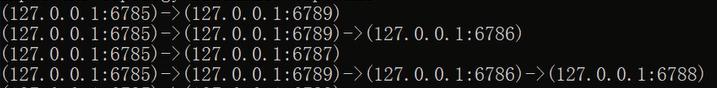
\includegraphics[scale=1]{imgs/ospfTest1.PNG}
			\caption{OSPF测试样例一}
			\label{fig:ospfTest1}
		\end{figure}
		\begin{figure}[H]
			\centering
			\includegraphics[scale=0.4]{imgs/topo2/topo2.png}
			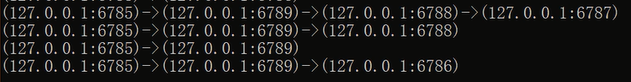
\includegraphics[scale=1]{imgs/ospfTest2.PNG}
			\caption{OSPF测试样例二}
			\label{fig:ospfTest2}
		\end{figure}
		成功找出了其中的最短路径。
	% subsection 结果 (end)
	\subsection{总结} % (fold)
	\label{sub:总结}
		% TODO 和真正OSPF协议的区别
		\begin{itemize}
			\item 本项目中实现的基本OSPF协议淡化了其区域概念,简化了报文类型和路由器类型,同时也简化了路由器状态。
			\item 原生的LS算法会导致路由震荡和路由循环问题,而我们实现的OSPF协议改善甚至基本解决了这类问题。
		\end{itemize}
		
% subsection 总结 (end)
	

% section ospf (end)

\section{基本中心化路由协议}
\subsection{协议概述} % (fold)
	\label{sub:协议概述}
		中心化路由协议是一个基于链路状态的网络层路由协议,使用的是Dijkstra算法,该协议中定义了一个服务器,负责接收区域内运行该协议的路由器的链路信息并且根据这些信息计算出整个区域内路由器的最短路径树,构造出每个路由器的转发表,并发送给对应路由器。并且在服务器中能够获取指定路由器对的最短路径。
	% subsection 协议概述 (end)
	\subsection{算法} % (fold)
	\label{sub:算法}

	% subsection 算法 (end)
	\subsection{协议特性} % (fold)
	\label{sub:协议特性}
		\subsubsection{协议流程} % (fold)
		\label{ssub:协议流程}
			\begin{enumerate}
				\item 路由器加入某个区域后,向邻居发送hello报文,并将定期发送hello报文。
				\item 路由器定期向服务器发送LS报文,服务器接收后计算对应信息并定时向路由器发送转发表。
				\item 服务器和路由器都有失效机制,当应当发送信息的路由器在一段时间没有发送信息后将其置为失效。
			\end{enumerate}
		% subsubsection 协议流程 (end)
	% subsection 协议特性 (end)
	\subsection{报文格式} % (fold)
	\label{sub:报文格式}
		基本Centralized协议中包含的报文格式有hello报文、LS报文、转发表报文三种报文格式。
		\par LS 报文:
		\begin{table}[H]
		\centering
			\begin{tabular}{|c|}
				\hline
				Command \\
				\hline
				Source address \\
				\hline
				Destination address \\
				\hline
				Metric \\
				\hline
				Repeat of last 8 bytes \\
				\hline
				$\cdots$ \\
				\hline
			\end{tabular}		
		\end{table}
		\par Forward Table 报文:
		\begin{table}[H]
		\centering
			\begin{tabular}{|c|}
				\hline
				Command \\
				\hline
				Destination address \\
				\hline
				nextHop \\
				\hline
				Repeat of last 12 bytes \\
				\hline
				$\cdots$ \\
				\hline
			\end{tabular}		
		\end{table}
		\par Hello 报文:
		\begin{table}[H]
		\centering
			\begin{tabular}{|c|}
				\hline
				Command        \\
				\hline
				Source address \\
				\hline
				Metric         \\
				\hline
			\end{tabular}
		\end{table}
		\par 普通报文:
		\begin{table}[H]
		\centering
			\begin{tabular}{|c|}
				\hline
				Command \\
				\hline
				source address \\
				\hline
				destination address \\
				\hline
				payload \\
				\hline
			\end{tabular}		
		\end{table}
		\par 报文项解释:
		\begin{enumerate}
			\item Command(1 Byte):指明这条报文的类型。
				\begin{enumerate}[]
					\item 0: 普通报文
					\item 1:hello
					\item 2:LS
					\item 3:转发表
				\end{enumerate}
			\item Source address(6 Bytes):指明发送方的源地址和监听端口。
			\item Destination address(6 Bytes):指明目的地的源地址和监听端口。
			\item nextHop(6 Bytes):下一跳IP地址和监听端口。
			\item Metric(2 Bytes):代价度量。
		\end{enumerate}
			
	% subsection 报文格式 (end)
	\subsection{协议扩展} % (fold)
	\label{sub:协议扩展}
		查找路径功能。在服务器中,实现了指定路由器对查找两者之间的最短路径的功能。
	% subsection 协议扩展 (end)
	\subsection{协议实现} % (fold)
	\label{sub:协议实现}
		\begin{enumerate}
			\item 客户端程序使用python编写,主要使用的是socket、threading等库。
			\item 使用Twisted异步编程框架编写服务器端。使用Twisted框架编写的服务器端具有低功耗、资源利用率高的特点,同时事件驱动的内在逻辑也符合该服务器的功能特性。
		\end{enumerate}
	% subsection 协议实现 (end)
	\subsection{结果} % (fold)
	\label{sub:结果}
		测试结果如下图\ref{fig:CentralizedTest1}和\ref{fig:CentralizedTest2}所示:
		\begin{figure}[H]
			\centering
			\includegraphics[scale=0.4]{imgs/topo3/tpop1.png}
			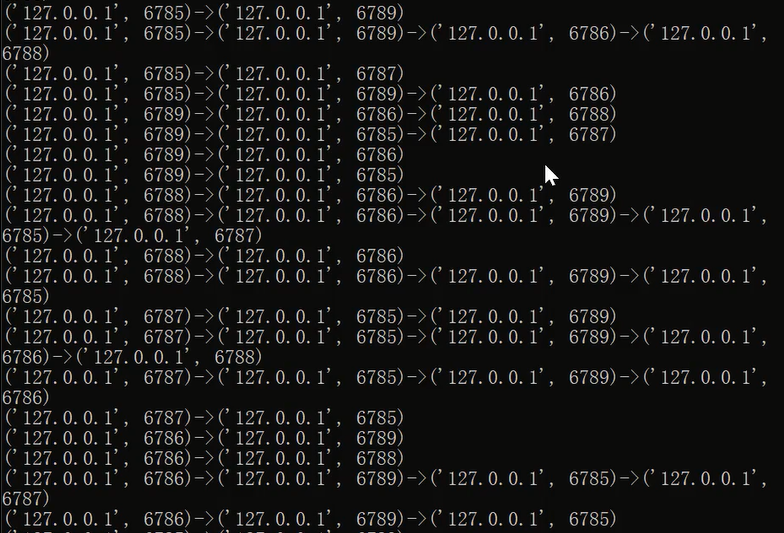
\includegraphics[scale=1]{imgs/cenTest1.PNG}
			\caption{中心化路由测试样例一}
			\label{fig:CentralizedTest1}
		\end{figure}
		\begin{figure}[H]
			\centering
			\includegraphics[scale=0.4]{imgs/topo3/topo2.png}
			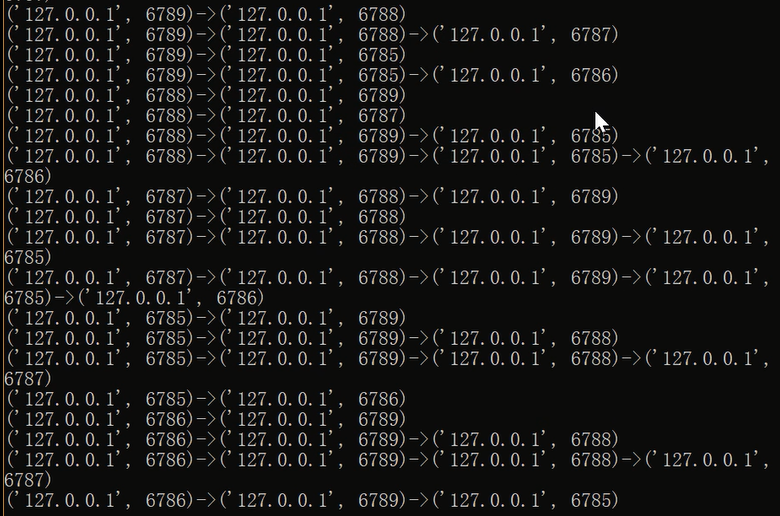
\includegraphics[scale=1]{imgs/cenTest2.PNG}
			\caption{中心化路由测试样例二}
			\label{fig:CentralizedTest2}
		\end{figure}
		成功找出了全部最短路径。
	% subsection 结果 (end)
	\subsection{总结} % (fold)
	\label{sub:总结}
		\begin{enumerate}
			\item 由于在中心化路由协议中每个路由器的转发表都是由服务器计算并且同时几乎获得,即转发表基于同一张图结构,则不存在路由循环、路由震荡等问题。
			\item 但是中心化路由协议具有滞后性,虽然该滞后性也使得路由更加稳定,但是不能及时地检测到路由的变化,造成某些数据报文发送的浪费。
		\end{enumerate}
	% subsection 总结 (end)
% section Centralized (end)

\section{安装与部署} % (fold)
\label{sec:安装与部署}

% section 安装与部署 (end)

\section{项目管理记录} % (fold)
\label{sec:项目管理记录}

% section 项目管理记录 (end)

\section{总结} % (fold)
\label{sec:总结}
	\subsection{关于在应用层模拟网络层} % (fold)
	\label{sub:关于在应用层模拟网络层协议}
	
	% subsection 关于在应用层模拟网络层 (end)
% section 总结 (end)




\newpage
\begin{appendices}
    \section{参考文献} % (fold)
        \begin{enumerate}
        \item RFC2328, Open Shorst Path First Protocol.
        \item RFC2453, Route Information Protocol.
        \item \url{https://en.wikipedia.org/wiki/Open_Shortest_Path_First}, Wikipedia for OSPF.
        \item \url{https://en.wikipedia.org/wiki/Routing_Information_Protocol}, Wikipedia for RIP.
        \item \url{http://www.clnchina.com.cn/discussion_forum/2010/0721/8402.shtml}, Four Timer in RIP.
        \end{enumerate}
    % section  (end)
\end{appendices}

\end{document}